\section{Tuesday, November 22th}
\subsection{Steady-State/Transient Response}
Today we will start with one way of splitting the output of a system.\\
Specifically we will split this into a component that persists in time -- steady-state -- and a component that dies out.

Given the following difference equation:
\begin{align*}
    y(n)
    &= \alpha y(n-1) + x(n)\quad|\alpha|<1
    \\
    x(n) &= u(n)\quad\text{System is initially at rest}
    \\
    \Yhat 
    &= \Xhat\Hhat
    \\
    \Yhat 
    &=\alpha z^{-1} \Yhat + \Xhat\implies(1-\alpha z^{-1})\Yhat=\Xhat
    \\
    \Hhat
    &=\frac{\Yhat}{\Xhat}=\frac{1}{1-\alpha z^{-1}}=\frac{z}{z-\alpha},\quad|\alpha|<|z|
    \\
    \Yhat
    &=\frac{z}{z-1}\frac{z}{z-\alpha}
    \\
    &=z\left[\frac{1}{z-1}\frac{z}{z-\alpha}\right]
    =z\left[\frac{z}{(z-1)(z-\alpha)}\right]
    \\
    &= \frac{A}{z-1}+\frac{B}{z-\alpha}
    \\
    &= \underbrace{\frac{1}{1-\alpha}}_{A}\frac{1}{z-1}\underbrace{-\frac{\alpha}{1-\alpha}}_B\frac{1}{z-\alpha}
    \\
    \therefore\Yhat 
    &=z\left[\frac{z}{(z-1)(z-\alpha)}\right]
    \\
    &= {\frac{1}{1-\alpha}}\frac{1}{z-1}{-\frac{\alpha}{1-\alpha}}\frac{1}{z-\alpha},\quad1<|z|
    \\
    &\mathcal Z^{-1}\downarrow
    \\
    y(n)
    &=\underbrace{\frac{1}{1-\alpha}u(n)}_{y_{SS}(n) \text{persists}} - \underbrace{\frac{\alpha}{1-\alpha}\alpha^n u(n)}_{y_{TR}(n)}
    \\
    \lim_{n\to\infty} y_{TR}(n) &= 0
\end{align*}
where we work entirely in the $z$-domain.

The ROC of the system expands outwards from $z=\alpha$ and the unit step has ROC of $1<|z|$ which leads to a non-trivial overlap.

Although we do not see it here, note that a pole/zero cancellation can actually make the ROC of the mixed transform be greater than the minimal intersection.

\begin{shaded}
Q: What's the response of the system to $x(n)=1\quad\forall n\in\mathbb Z$?
\end{shaded}
\textit{Hint:}\[
\beta_{}^n u(n) \zt \frac{1}{1-\beta z^{-1}}, \quad|\beta|<|z|
\]

A: If we plug in $z_0^n=1$ to our system then we get $\Hhat =\frac{z}{z-\alpha},\quad|\alpha|<|z|$ to get output $\frac{1}{1-\alpha}$.

Note that this is the same as $\displaystyle\lim_{n\to\infty} y(n) = \frac{1}{1-\alpha}$.

\hrulefill

\begin{shaded}
What's the response to the input $x(n)=\cos(\omega_0 n)u(n)$?
\end{shaded}
\begin{align*}
    x(n) 
    &=\frac{1}{2} e^{i \omega_0^n} u(n)+\frac{1}{2} e^{-i \omega_0 n} u(n) \\
    \beta^n u(n) \rightarrow \boxed{h(n)=\alpha^n u(n)}& \rightarrow {A \beta^n u(n)}+{B \alpha^n u(n)}
\end{align*}

Everything in this lecture so far has assumed that the system is initially at rest.

\hrulefill

\subsection{Systems not initially at rest}
Given a Causal, BIBO Stable, System. Note that we do not care about the history before the initial state as the initial state tells us all we need to know:
\begin{align*}
    y(n)
    &= \alpha y(n-1)+x(n),\quad|\alpha|<1
    \\
    y(-1)
    &\neq 0;\quad \ x(n)=0,\quad n\ge0
    \\
    y(0)
    &=\alpha y(-1)
    \\
    y(1)
    &=\alpha y(0)=\alpha^2 y(-1)
    \\
    y(2)
    &=\alpha y(1)=\alpha^3 y(-1)
    \\
    \implies
    y_{ZIR}(n)
    &=\alpha^{n+1} y(-1)
    \\
    \text{Now, let } y(-1)
    &=0,\ x(n)=u(n)
    \\
    y_{ZSR}(n)
    &=
    {\frac{1}{1-\alpha}u(n)} - {\frac{\alpha}{1-\alpha}\alpha^n u(n)}
\end{align*}
\begin{shaded}
What's the response if $y(-1)\neq0\quad\&\quad x(n)=u(n)$?
\end{shaded}
\begin{align*}
    y(n)
    &= y_{ZIR}(n) + y_{ZSR}(n)
    \\
    &= \underbrace{\alpha^{n+1}y(-1)}_{y_{ZIR}(n)}
    + \underbrace{\frac{1}{1-\alpha}u(n) - \frac{\alpha}{1-\alpha}\alpha^n u(n)}_{y_{ZSR}(n)}
\end{align*}
\hrulefill
\begin{align*}
    y(n)
    &=
    \alpha y(n-1) + x(n)
    \\
    y(n) u(n)
    &=
    \alpha y(n-1)u(n) + x(n)u(n)
    \\
    \sum_{n=-\infty}^{\infty} y(n) u(n)\zn
    &=
    \alpha \sum_{n=-\infty}^{\infty} y(n-1)u(n)\zn + \sum_{n=-\infty}^{\infty} x(n)u(n)\zn
    \\
    \sum_{n=0}^{\infty} y(n) \zn
    &=
    \alpha \sum_{n=-0}^{\infty} y(n-1)\zn + \sum_{n=0}^{\infty} x(n)\zn
    \\
    \Yhatu
    &=
    \alpha \sum_{n=-0}^{\infty} y(n-1)\zn + \Xhatu
    &&\text{[Unilateral Z Transform]}
    \\
    \text{Lemma: }
    \sum_{n=0}^{\infty} y(n-1) \zn
    &=
    \sum_{m=-1}^{\infty} y(m) z^{-(m+1)}
    = y(-1) + \zinv \Yhatu
    &&\text{[Change of Variables]}
    \\
    &
    &&\text{[$m=n-1\implies n=m+1$]}
    \\
    \hat{y}(z) &=\frac{\alpha y(-1)}{1-\alpha z^{-1}}+\frac{\hat{x}(z)}{1-\alpha z^{-1}} \\
    &=\alpha y(-1) \frac{1}{1-\alpha z^{-1}}+\hat{x}(z) \frac{1}{1-\alpha z^{-1}} \\
    \hat{y}(z) &=\alpha y(-1) \hat{H}(z)+\underbrace{\hat{x}(z) \hat{H}(z)}_{\text{Done Before}}
    \\
    y(n)&= \alpha y(-1)h(n)+
    &&\text{[$h(n)=\alpha^{n}u(n)$]}
    \\
    y(n)&= \alpha y(-1)\alpha^{n}u(n)
    + \frac{1}{1-\alpha}u(n) - \frac{\alpha}{1-\alpha}\alpha^n u(n)
\end{align*}

\subsection{Zero-Input Response/Zero-State Response}
See lecture notes below.

\subsection{Equilization}
See lecture notes below.

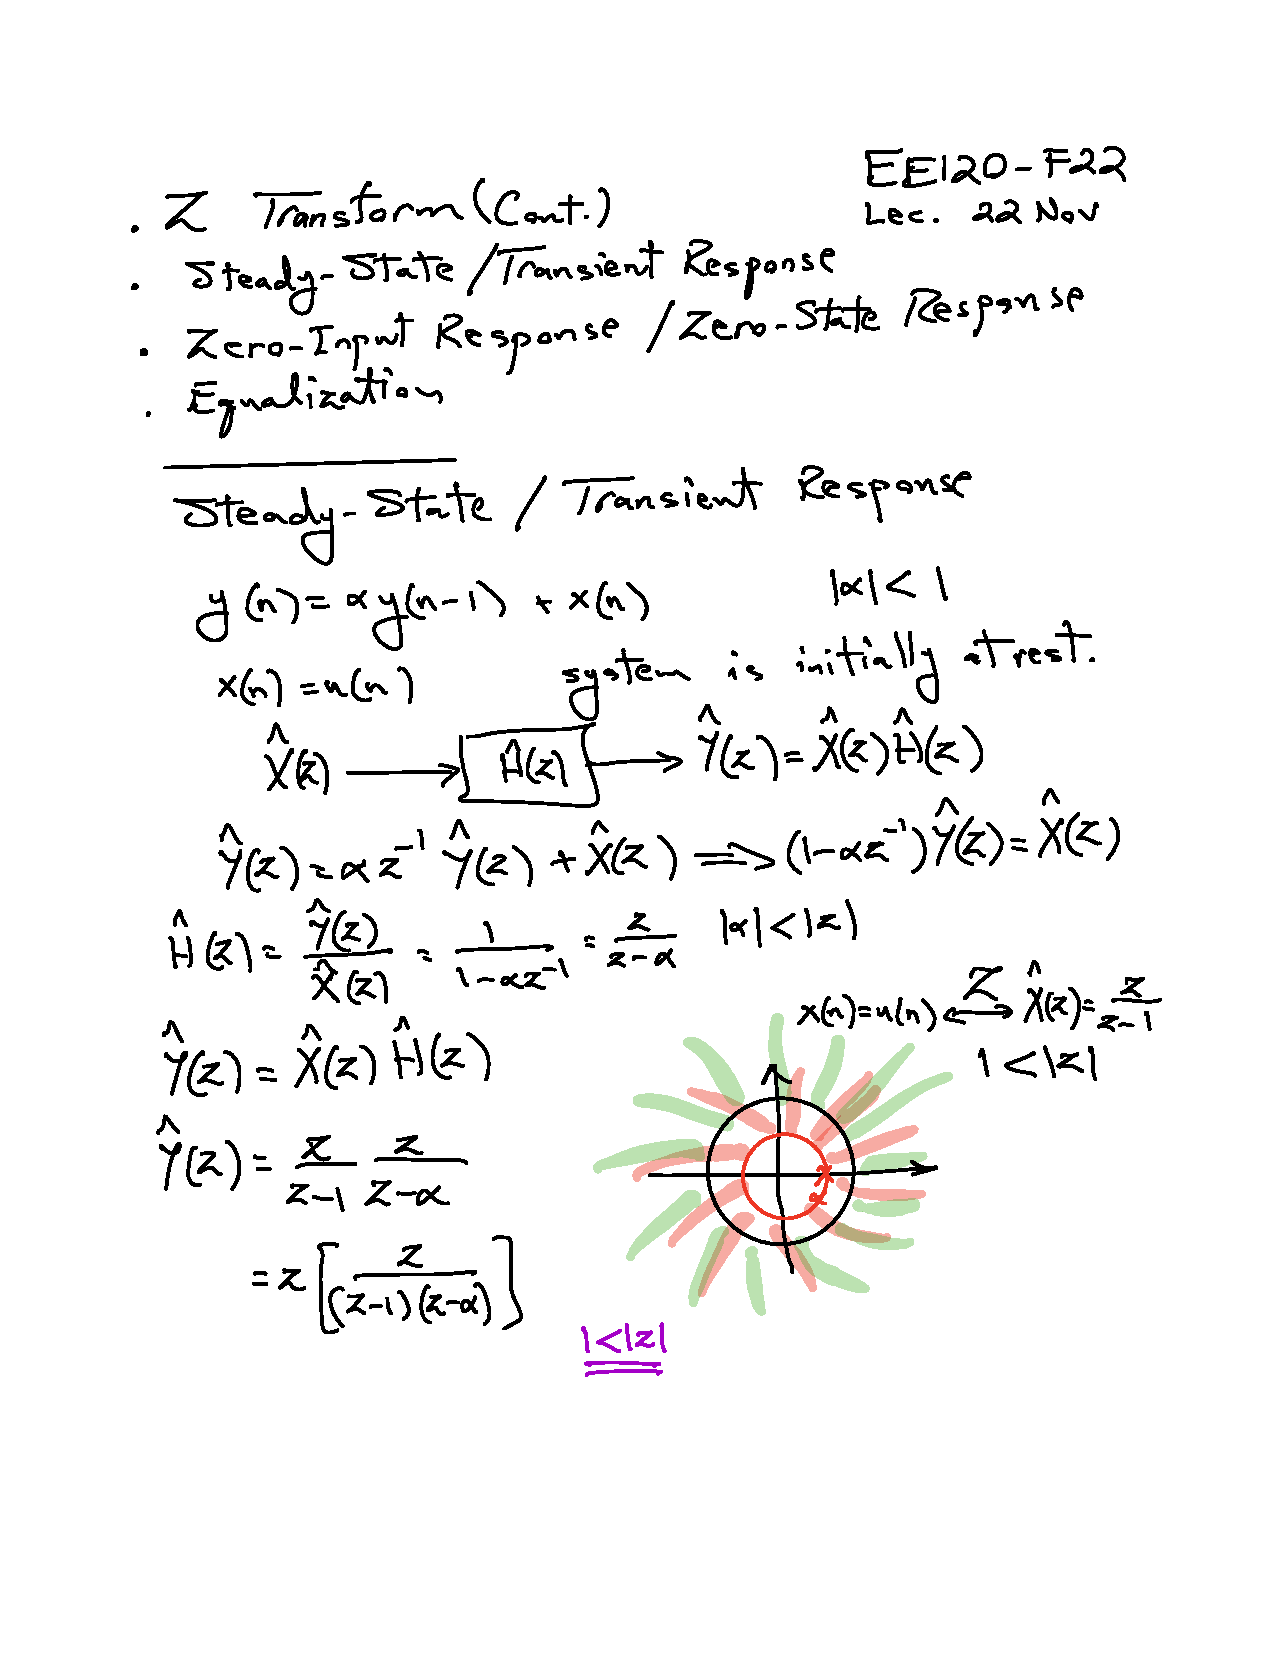
\includepdf[pages=-]{lectures/wk13/EE120-F22-L-2022-11-22-Z-Transform.pdf}
